\chapter{Linear approach}
\label{cha:LinearApproach}

Analyzing the main drawbacks of the reference papers concerning unsupervised segmentation methods, the first implemented approach aims to considerable reduce the computation steps. Unlike previous approaches, point correspondences are not seeked in order to segment the articulated object. Instead a segmentation is performed in order to find point correspondences. The approach operates straightforward, as it linearly subdivides an articulated object $M$ in two different configurations, referred to as $C_1$ and $C_2$, into sub clusters. The subdividing of those clusters proceeds until two matches can be detected (see section \ref{Subdividing}). Thereby, it is taken advantage of PCA to associate sub clusters of $C_1$ and $C_2$.

\section{Cluster detection by region growing}
\label{clustering}

As a first step, the resolution of $M$ is computed in order to have an indicator how to set the specific thresholds. Thus, 10 random points are selected from $M$ and the distance to their closest points are computed. Then the median value is taken as resolution to avoid distortion in case of outliers. Then, the initial goal is to remove possible noise and outliers to proceed the linear approach with the two clusters $C_1$ and $C_2$. This is achieved by applying region growing on all points of $M$. A cluster $C_i$ is grown from an unclustered point $\boldsymbol{p}_i(x,y)$. Another point $\boldsymbol{p}_j(x,y)$ is added to the cluster $C_i$ if the euclidean distance between them $d(\boldsymbol{p}_i, \boldsymbol{p}_j)$ is below a predefined threshold $\tau$. The threshold is thereby depending on the resolution of $M$. As a next step, all points of $C_i$ are iteratively compared to the remaining unclustered points to allow the cluster to further grow. Once, all points of $C_i$ have been treated and no further points are added to the cluster, any unclustered point is used as a seed to grow another cluster $C_j$. If there are no unclustered points left, the cluster with the highest number of points $n$ is selected as input cluster for the segmentation algorithm. The remaining clusters are classified as noise and rejected for further computations. The region growing is performed for both configurations of $M$ in order to proceed the segmentation with the clusters $C_1$ and $C_2$ (see figure \ref{fig:pc_2parts}). 
%%
\begin{figure}[H]
	\centering\small
	\begin{tabular}{cc}
		\fbox{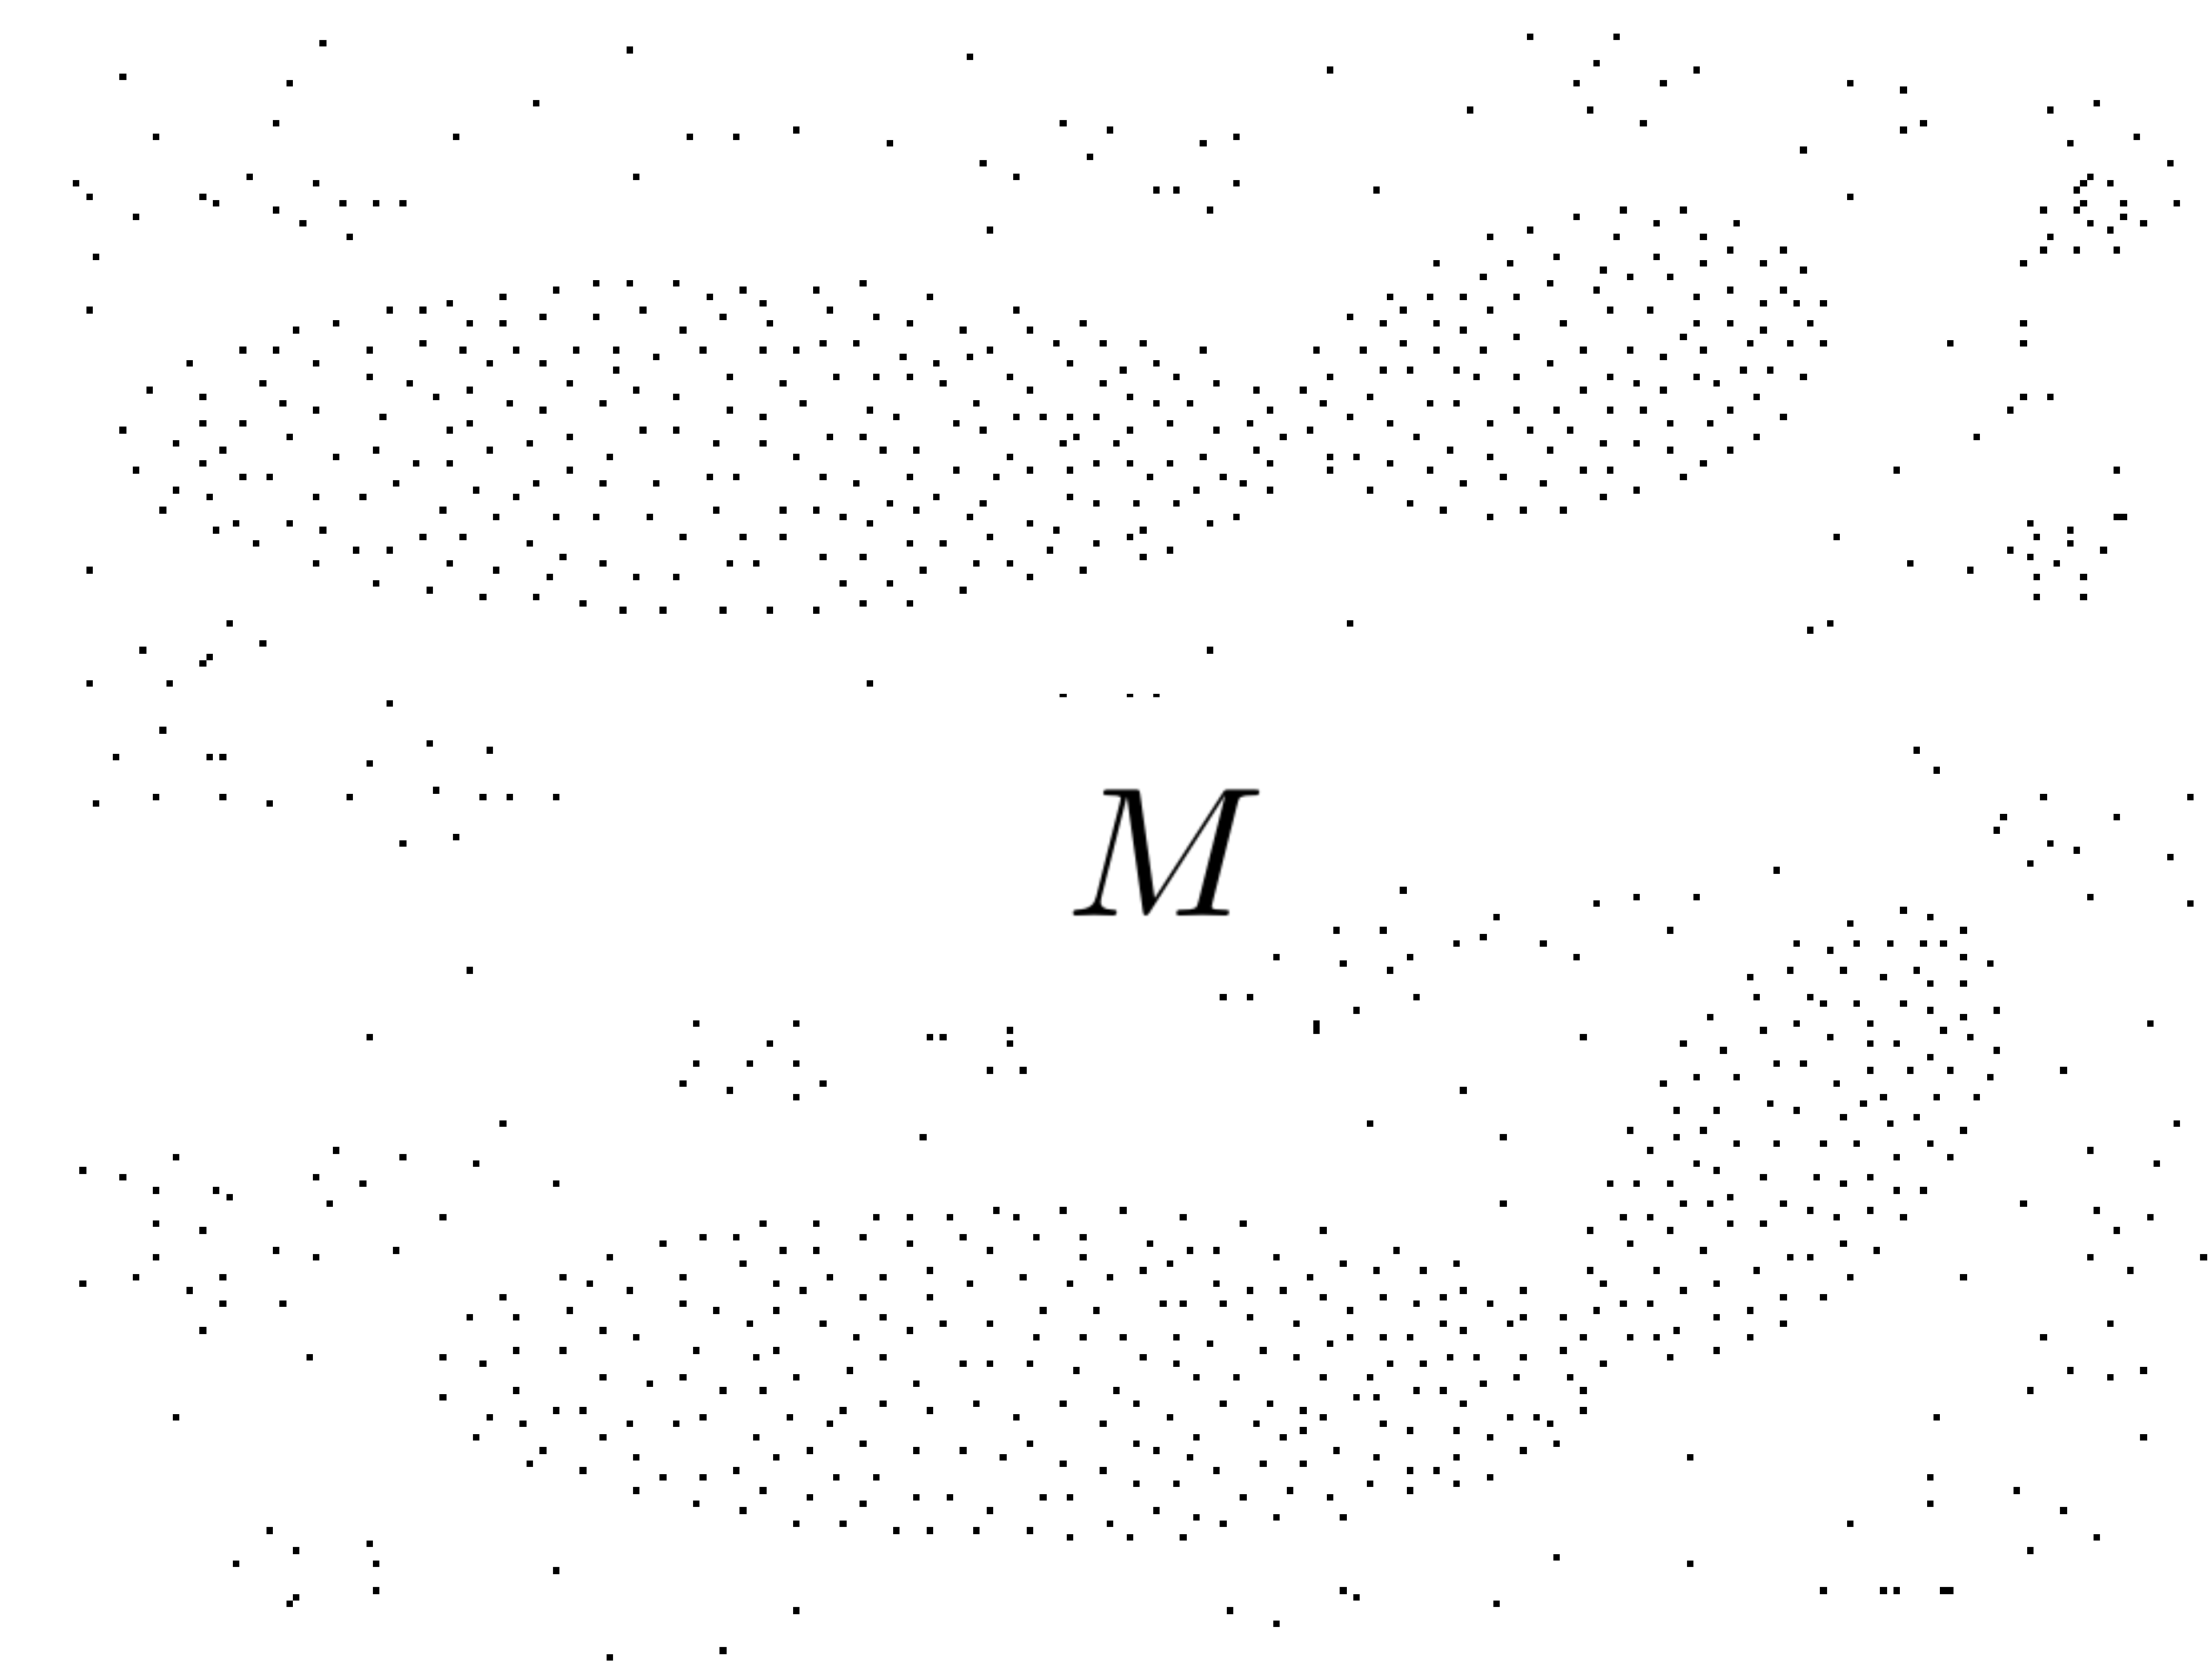
\includegraphics[width=0.45\textwidth]{pc_2parts_Noise}} &		
		\fbox{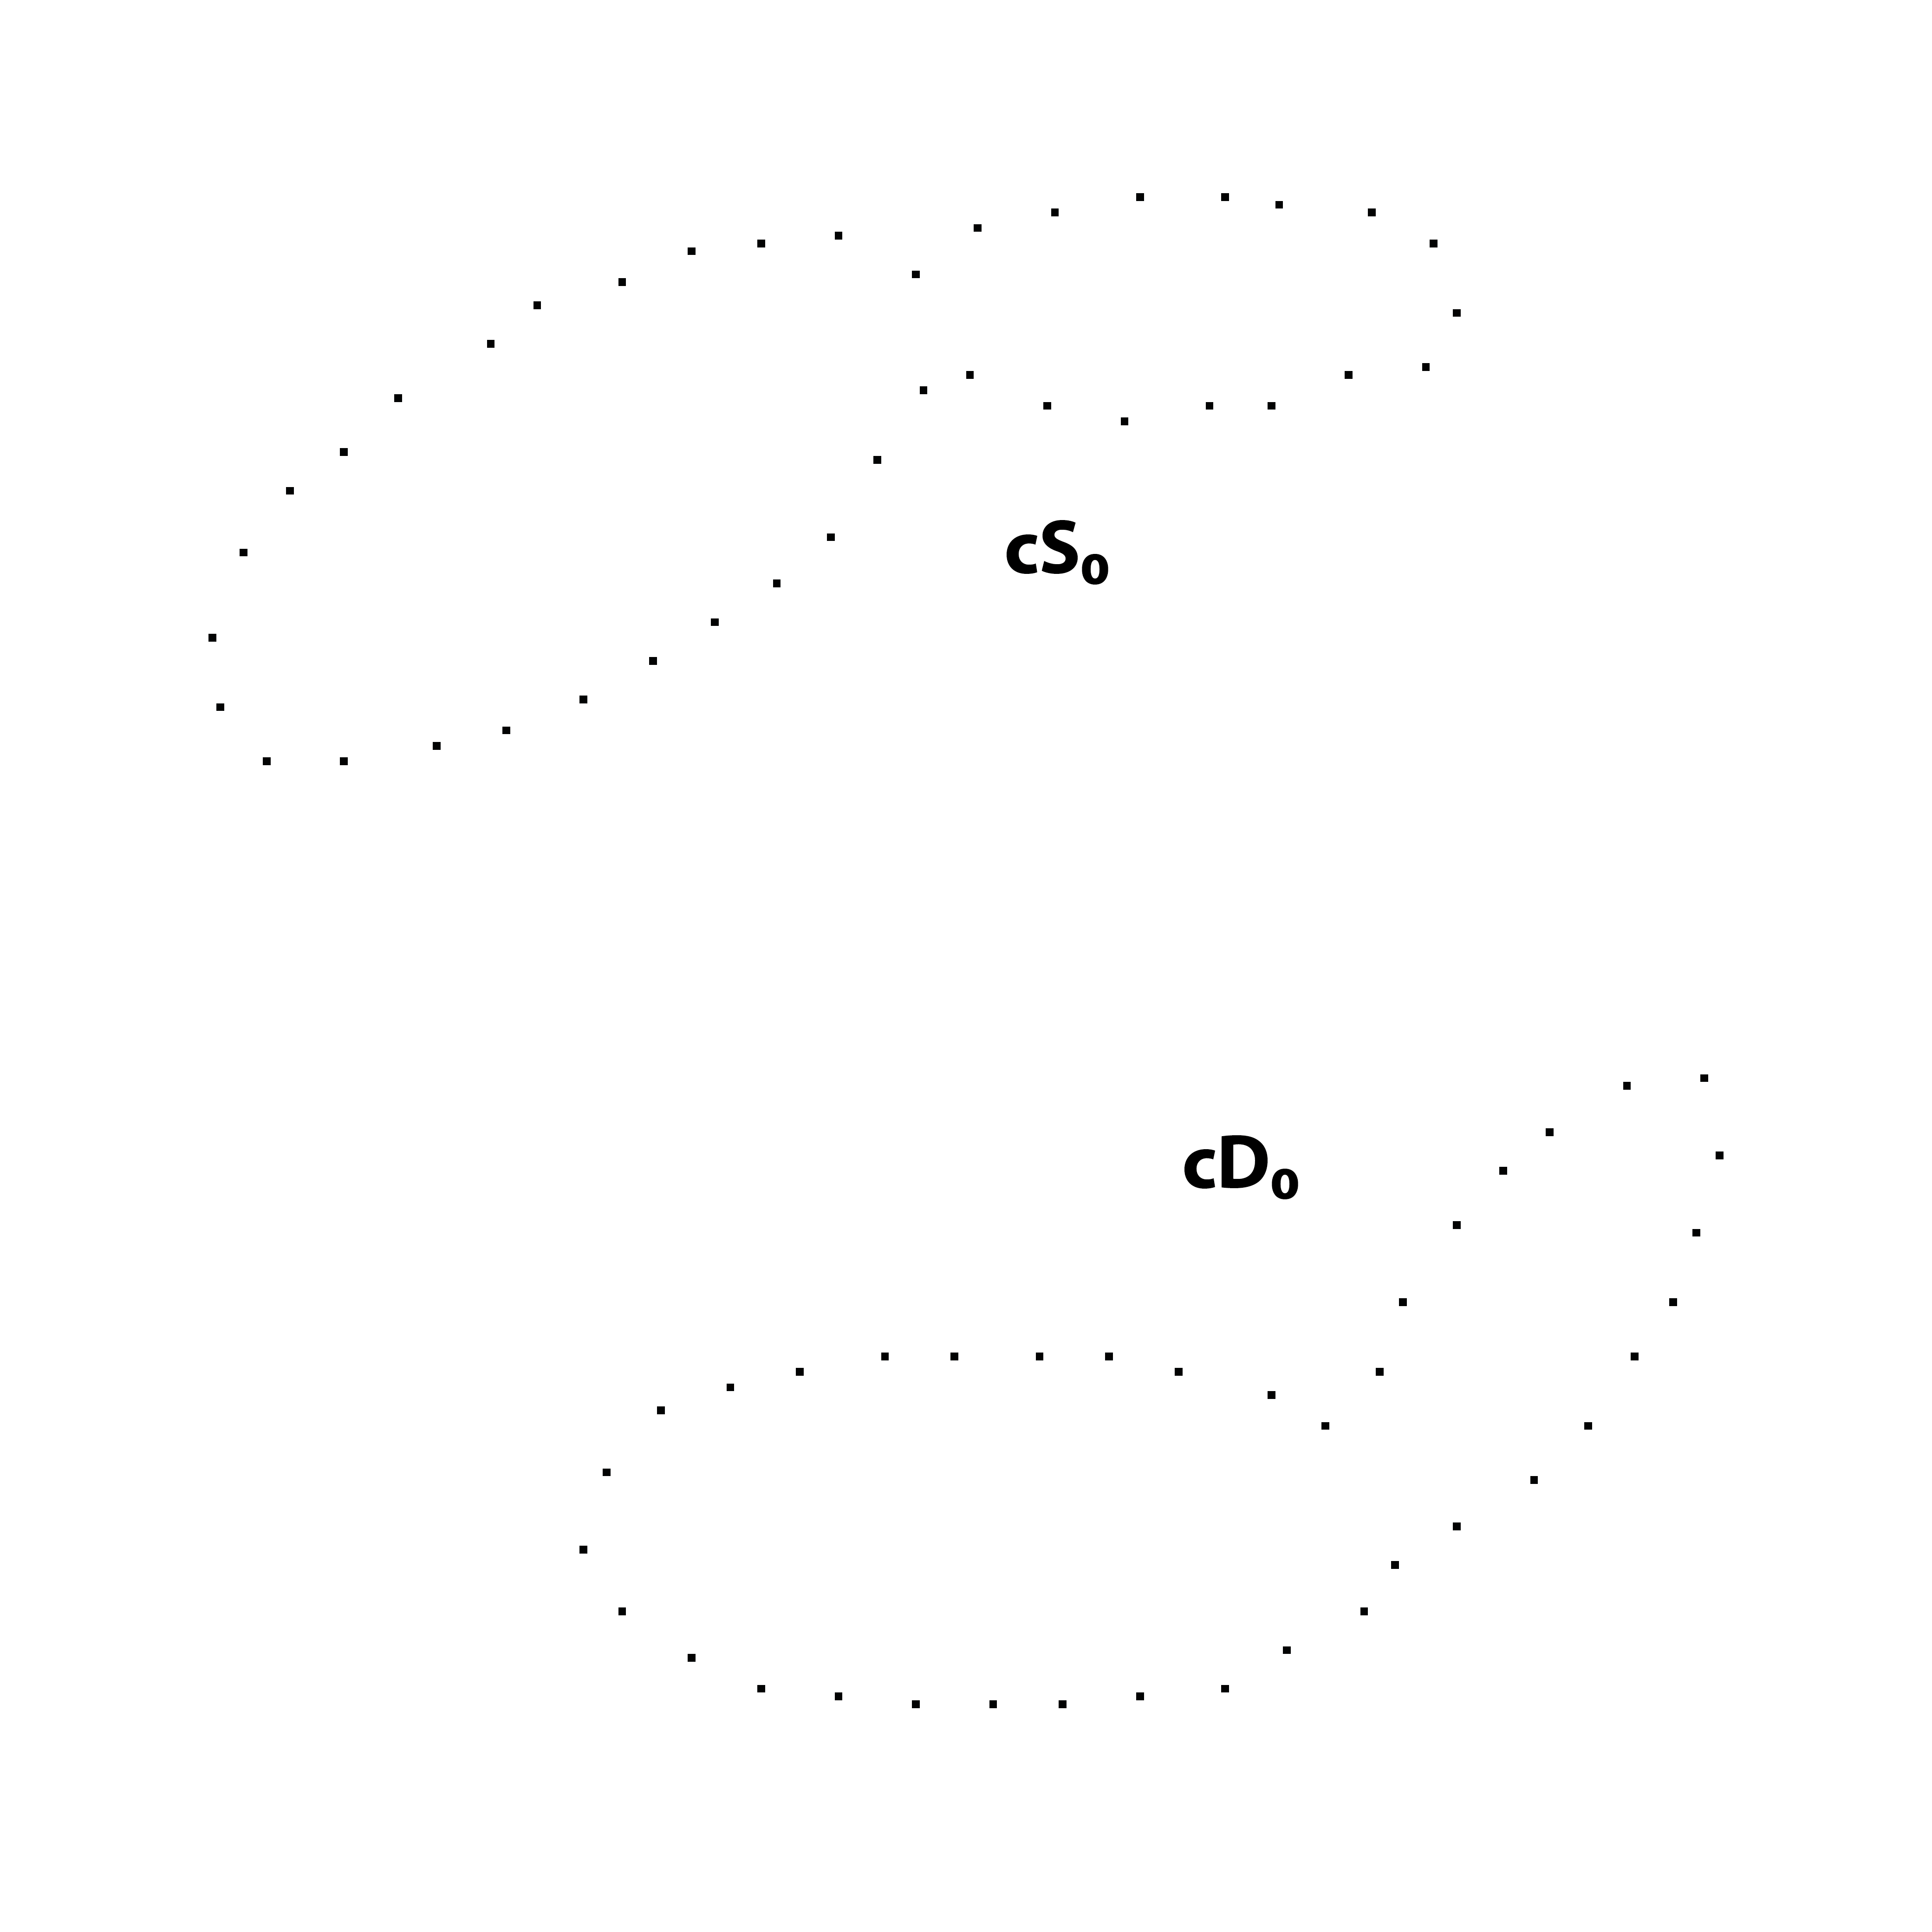
\includegraphics[width=0.45\textwidth]{pc_2parts_noNoise}} 
		\\
		(a) & (b) 
	\end{tabular}
	\caption{Taking a mesh $M$ in two different poses as input (a), removing noise of the input point clouds (b) to achieve the input clusters $C_1$ and $C_2$.} 
	\label{fig:pc_2parts}
\end{figure}

\section{Subdividing into clusters}
\label{Subdividing}
As a first step of the subdividing process, the principal axes $p_{1}$ and $p_{2}$ of $C_1$ and $C_2$ are computed. Those are required to offer a similar divider position base for the subdividing procedure. For that, the orientation $\theta$ of $C_1$ and $C_2$ are computed by calculating the central moments
%%
\begin{equation}
\mu_{pq}(\mathcal{C}) = \sum_{(x,y)\in\mathcal{C}} (x - \bar{x})^p \cdot (y - \bar{y})^q
\end{equation}
%%
\begin{equation}
\theta(\mathcal{C}) = \frac{1}{2} \tan^{-1} \left(\frac{2\cdot \mu_{11}(\mathcal{C})}{\mu_{20}(\mathcal{C}) - \mu_{02}(\mathcal{C})}\right)
\end{equation}
%%
for all clusters $\mathcal{C}$. The divider positions are then determined by computing the perpendicular secondary axes $s_{1}$ and $s_{2}$ to $p_{1}$ and $p_2$ through the centroids. The secondary axes divide $C_1$ and $C_2$ into the sub clusters $C_{1,1}$ and $C_{1,2}$ as well as $C_{2,1}$ and $C_{2,2}$. The association of clusters between $C_1$ and $C_2$ is determined by the sub clusters being located left or right of $s_1$ or $s_2$ (see figure \ref{fig:dc_axes_2p}). 
%%
\begin{figure}[H]
	\centering
	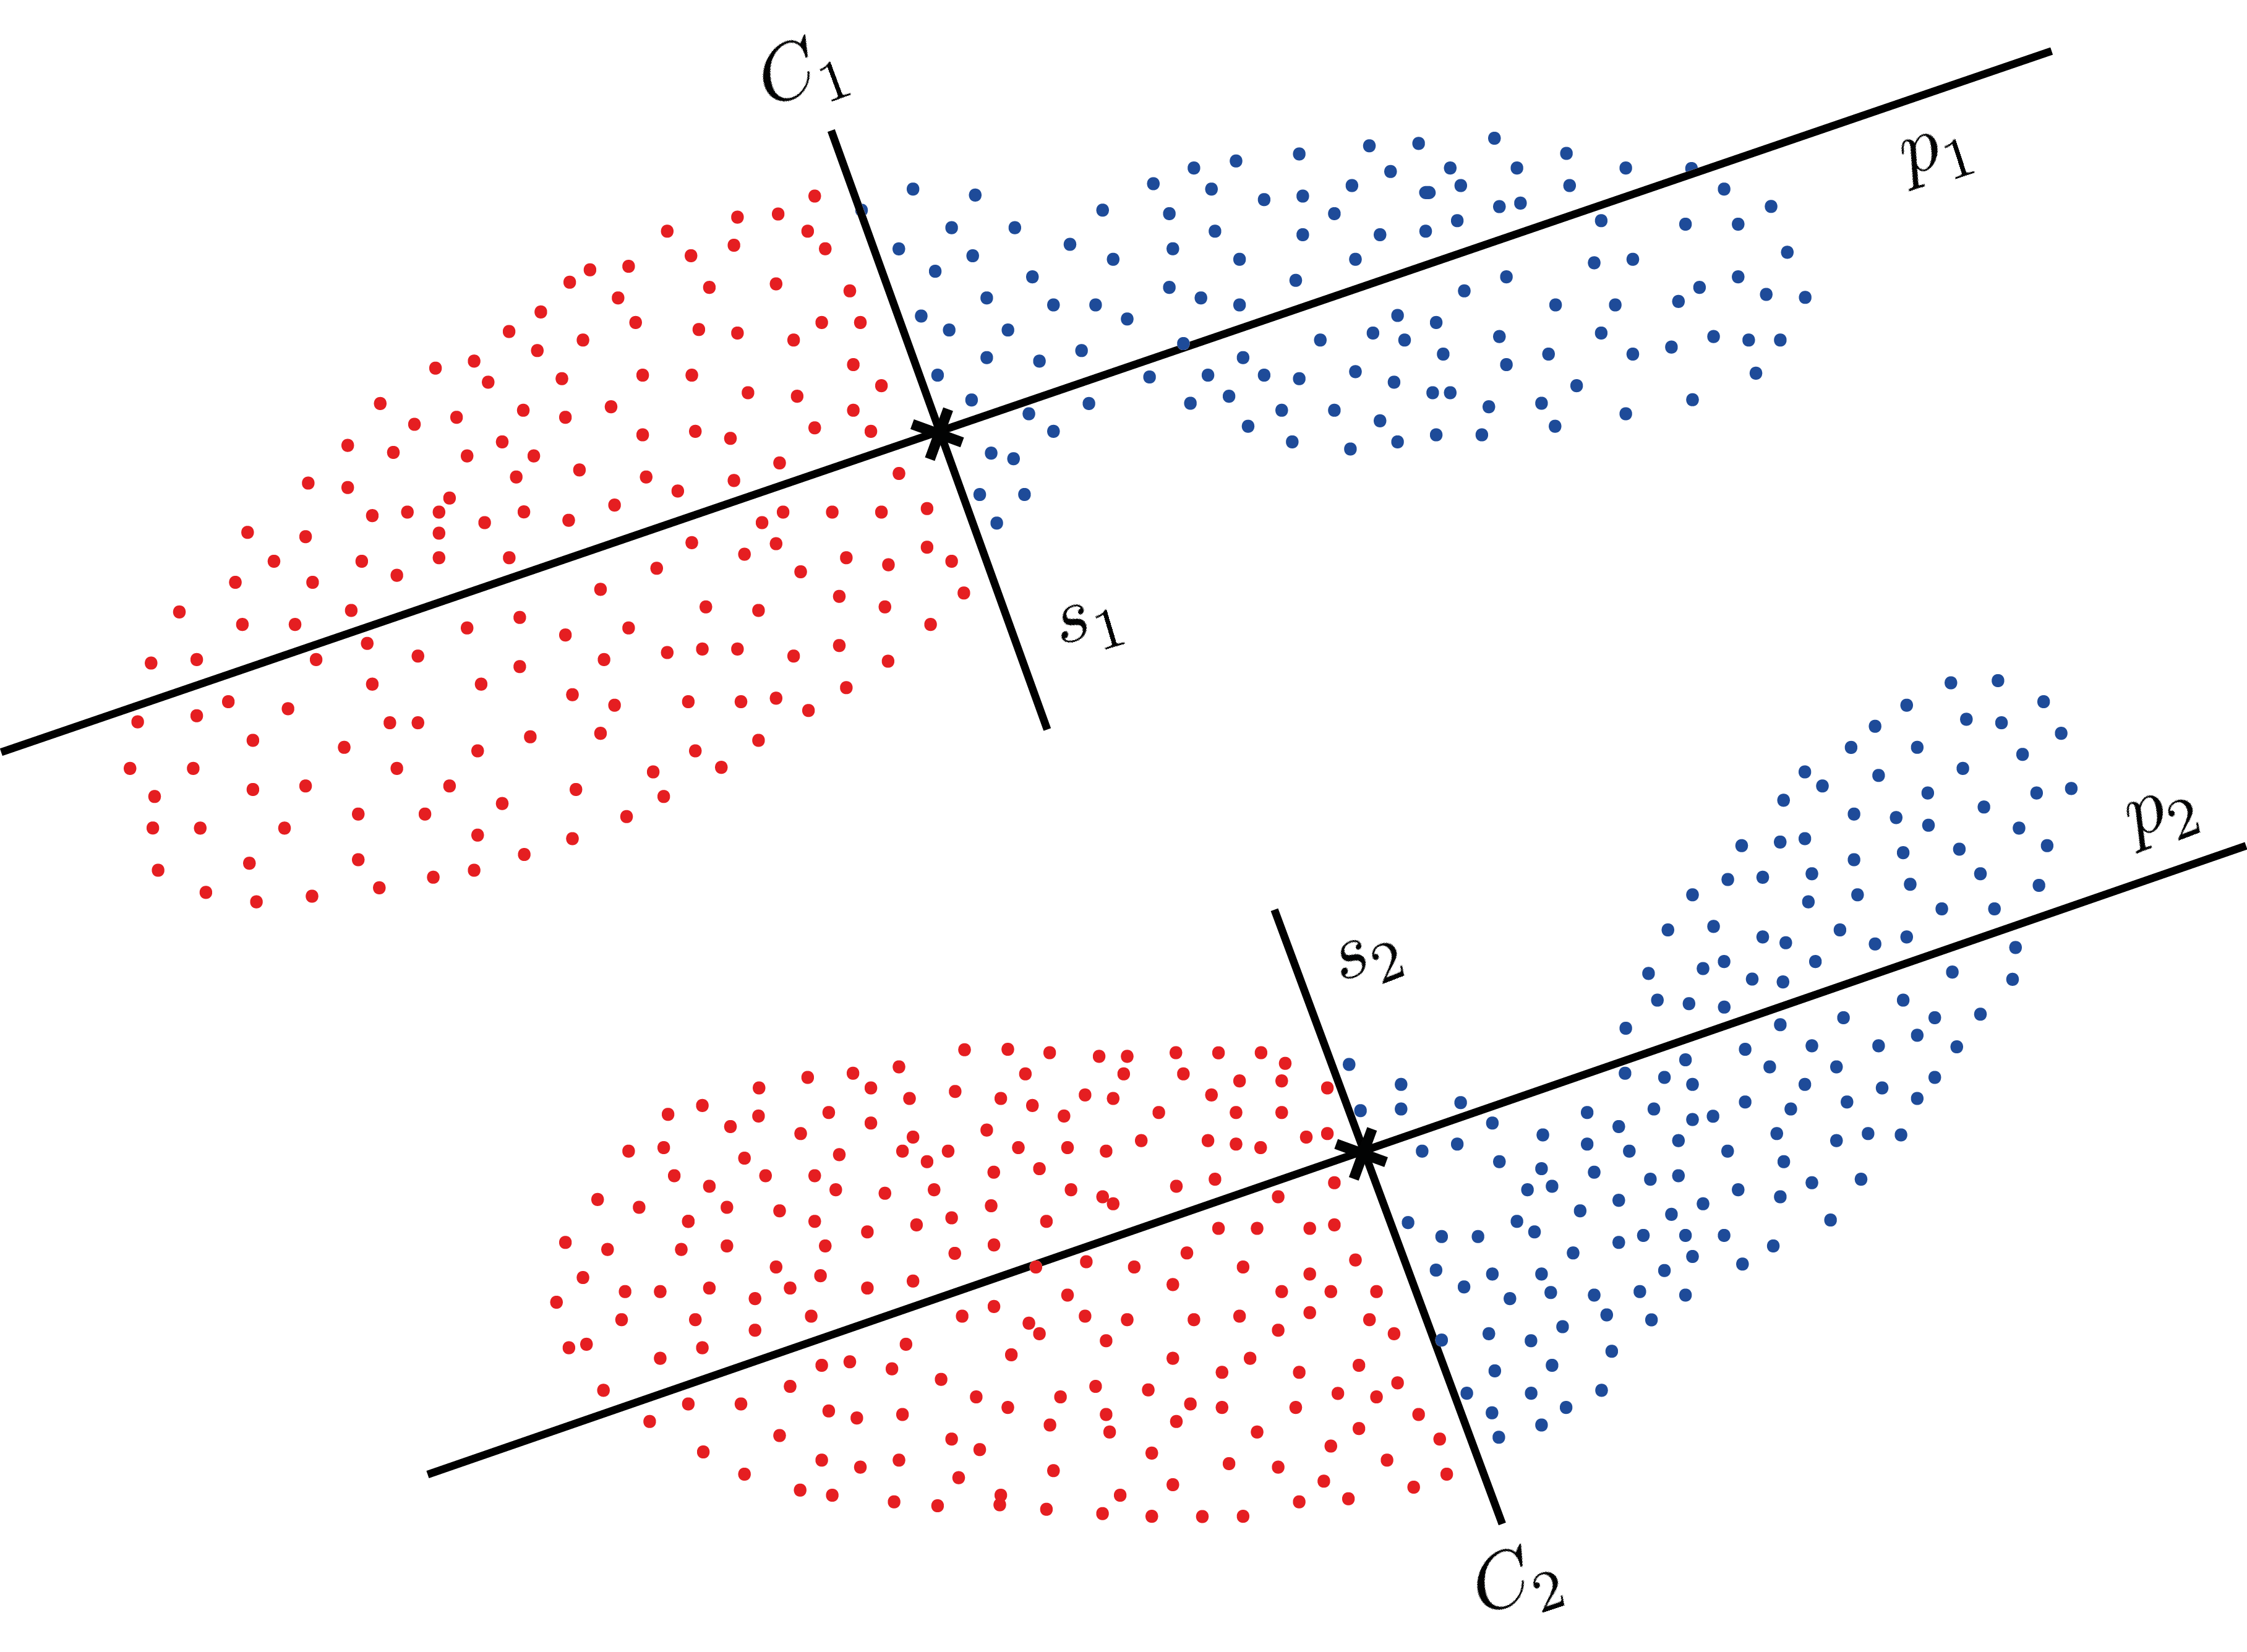
\includegraphics[width=0.7\linewidth]{illustration_axes}
	\caption{Subdividing $C_1$ and $C_2$ into two sub clusters by computing the secondary axes $s_1$ and $s_2$ perpendicular to $p_1$ and $p_2$ through the centroids. Associated clusters are colored in the same color, red for both left clusters and blue for both right clusters.}
	\label{fig:dc_axes_2p}
\end{figure}
%%
In each iteration step two related sub clusters are then verified to match. By applying the ICP on two associated clusters a certain matching error $e$ is computed between their cluster points $ C_p =  \{ p_1, \ldots, p_m\}$ and the associated points $ C_q =  \{ q_1, \ldots, q_m\}$. To eliminate the dependency between the matching error and the number of cluster points $m$, the average error per point of $C_p$ and $C_q$
%%
\begin{equation}
e_{\mathrm{avg}(C_p, C_q)} = \frac{1}{| C_p |} \cdot \displaystyle\sum_{i=0}^{m}\| \boldsymbol{p}_i - \boldsymbol{q}_i\|^2
\end{equation}
%%
is computed, assuming that the two clusters $C_p$ and $C_q$ contain the same number of cluster points $m$. In case of varying point amounts, excessive points are not considered in the error amount calculation. Two clusters $C_p$ and $C_q$ are stated to match, if $e_{avg} < \tau$. It is quite essential to determine an appropriate threshold $\tau$, which requires to take the resolution of the input data into account. In case of being overvalued, clusters are more likely to match which could result in insufficient subdividing. On the contrary, it becomes increasingly unlikely that clusters match, which will result in further subdividing and the detection of too many rigid parts. If the matching between two clusters does not succeed, they are both further subdivided into two sub clusters. The whole procedure is repeated recursively for all clusters $\mathcal{C} = (C_{i,1}, \ldots, C_{i,m})$ of $C_1$ and $C_2$ until all associated clusters of $C_1$ match the clusters of $C_2$. Matching sub clusters are stored in a list $\mathcal{L}$ sorted by their actual location resulting from a cluster tree (see subsection \ref{tree}).

\section{Merging sub clusters to rigid parts}
\label{mergingClusters}
%%
As a next step, adjacent sub clusters from $\mathcal{L}$ are iteratively merged and subsequently verified to still match. This process is required to rejoin, if necessary, segmented sub clusters to the rigid parts of the articulated object. This is the case, if a rigid part was subdivided during the previous subdividing step (see section \ref{Subdividing}). The merging initiates with the first set of associated sub clusters in the list ($L_{1,i}$, $L_{2,i}$) and their adjacent sub clusters ($L_{1,i+1},L_{2,i+1}$). If the resulting merged clusters can be matched in terms of the matching error $e_{avg}$, the merging proceeds with the adjacent cluster $L_{1,i+2},L_{2,i+2}$. If not, the merging is not executed and $L_{1,i}$, $L_{2,i}$ are stored in a list of resulting rigid parts $\mathcal{P}$. The merging procedure then initiates with $L_{1,i+1},L_{2,i+1}$. The process terminates if all clusters of $\mathcal{L}$ are verified and consequently all sub clusters are assigned to rigid parts $\mathcal{P} =  \{P_1,\ldots,P_m\}$ (see figure \ref{fig:clusterMerging}). 

%TODO: different image! --> too many clusters to only two clusters.

\begin{figure}
	\centering
	
\includegraphics[width=0.8\linewidth]{Placeholder}
	\caption{Detecting rigid parts of $C_1$ and $C_2$ by iteratively merging adjacent clusters of $\mathcal{L}$ that merged clusters still match.}
	\label{fig:clusterMerging}
\end{figure}

\section{Joint/skeleton estimation}

After detecting the rigid parts $\mathcal{P} =  \{ {P_1,\ldots,P_m}\}$, they joints linking them are estimated. As an initial approach the points of intersection between all principal axes of $\mathcal{P} = \{ {P_1,\ldots,P_m}\}$ are computed, which are determined to represent the joints. However, this calculation assumes that the rigid parts are symmetric, as in the other case the principal axes might not represent the skeleton of a rigid part. For this reason, another approach has to be taken into account. Anguelov \cite{Anguelov04} declares joints as two points of two neighboring rigid parts that undergo the same transformation $T$. In the current implementation a cluster point is only allocated to one rigid part $P$. An improvement of the current situation is therefore to select a number of closest points between neighboring rigid parts and computed the average point representing the joint (see figure \ref{fig:jointEstimation}). 
%%
%TODO: result joint estimation
%%
\begin{figure}
	\centering
	
\includegraphics[width=0.8\linewidth]{Placeholder}
	\caption{Detecting rigid parts of $C_1$ and $C_2$ by iteratively merging adjacent clusters of $\mathcal{L}$ that merged clusters still match.}
	\label{fig:jointEstimation}
\end{figure}
%%
\section{Implementation}
In order to primarily focus on an potential optimization of current segmentation approaches the proposed algorithm is implemented in 2D. The input for the segmentation is a 2D point cloud of an articulated object. Similar to 3D point clouds, it is represented by its surface, which is described by its hull. 

\subsection{Chosen environment}
As programming environment Java is chosen, using ImageJ\footnote{http://imagej.net} as image processing library. The environment depends on the following factors:
%%
\begin{itemize}
	\item familiarity and prior experience
	\item complexity
	\item availability of plug-ins for image processing
\end{itemize}
%%
As ImageJ is mainly used for 2D use cases, another implementation would be possible in 3D using PCL in C++ (see section \ref{3DImplementation}). As a result, the attention can be brought to 3D segmentation and visualization of articulated objects.

\subsection{Overview}
The algorithm was split into several java classes to separate the individual steps from the algorithm from each other. The starting point of the algorithm is represented by the class \texttt{Segmentation}. As input it solely requires a stack of two 2D images indicating the point clouds of a mesh $M$ in two different poses. As a first step, all clusters points are detected by iterating over the 2D images. A cluster point $\boldsymbol{p}_i(x,y)$ is determined by a pixel colored in black and is stored as \texttt{ClusterPoint} with its image coordinates. A class \texttt{Cluster} was implemented to store a cluster $C_i$ with all its points, its centroid, its resolution, the orientation $\theta$ as well as the principal and secondary axes $p_i$ and $s_i$. Next, possible noise is removed from the input meshes represented by the detected  cluster points. The result are two point clusters $C_1$ and $C_2$ which represent the articulated object in two poses. For the subdividing step (see section \ref{Subdividing}), a \texttt{ClusterTree} was implemented to simultaneously divide the main clusters $C_1$ and $C_2$ into sub clusters (see algorithm \ref{alg:subdivide}). Each node $N$ contains thereby two associated clusters $C_{1,i}$ and $C_{2,i}$. On two associated clusters from a node $N$ the \texttt{Registration} class is applied which registers them by taking advantage of ICP and Procrustes fitting. The recursive subdiving approach returnes a list of matching sub clusters which are subsequently merged to rigid parts (see algorithm \ref{alg:merging}). The \texttt{Visualization} class is responsible for displaying the clusters and rigid parts in different colors and draw PCA related components, like the axes and joints of the rigid parts. The \texttt{Matrix} class provides operations for performing transformations on clusters. An overview of the architecture can be seen on figure \ref{fig:UML}.
%%
%TODO: make new UML diagram! --> updated names + cluster points
\begin{figure} [H]
	\centering
	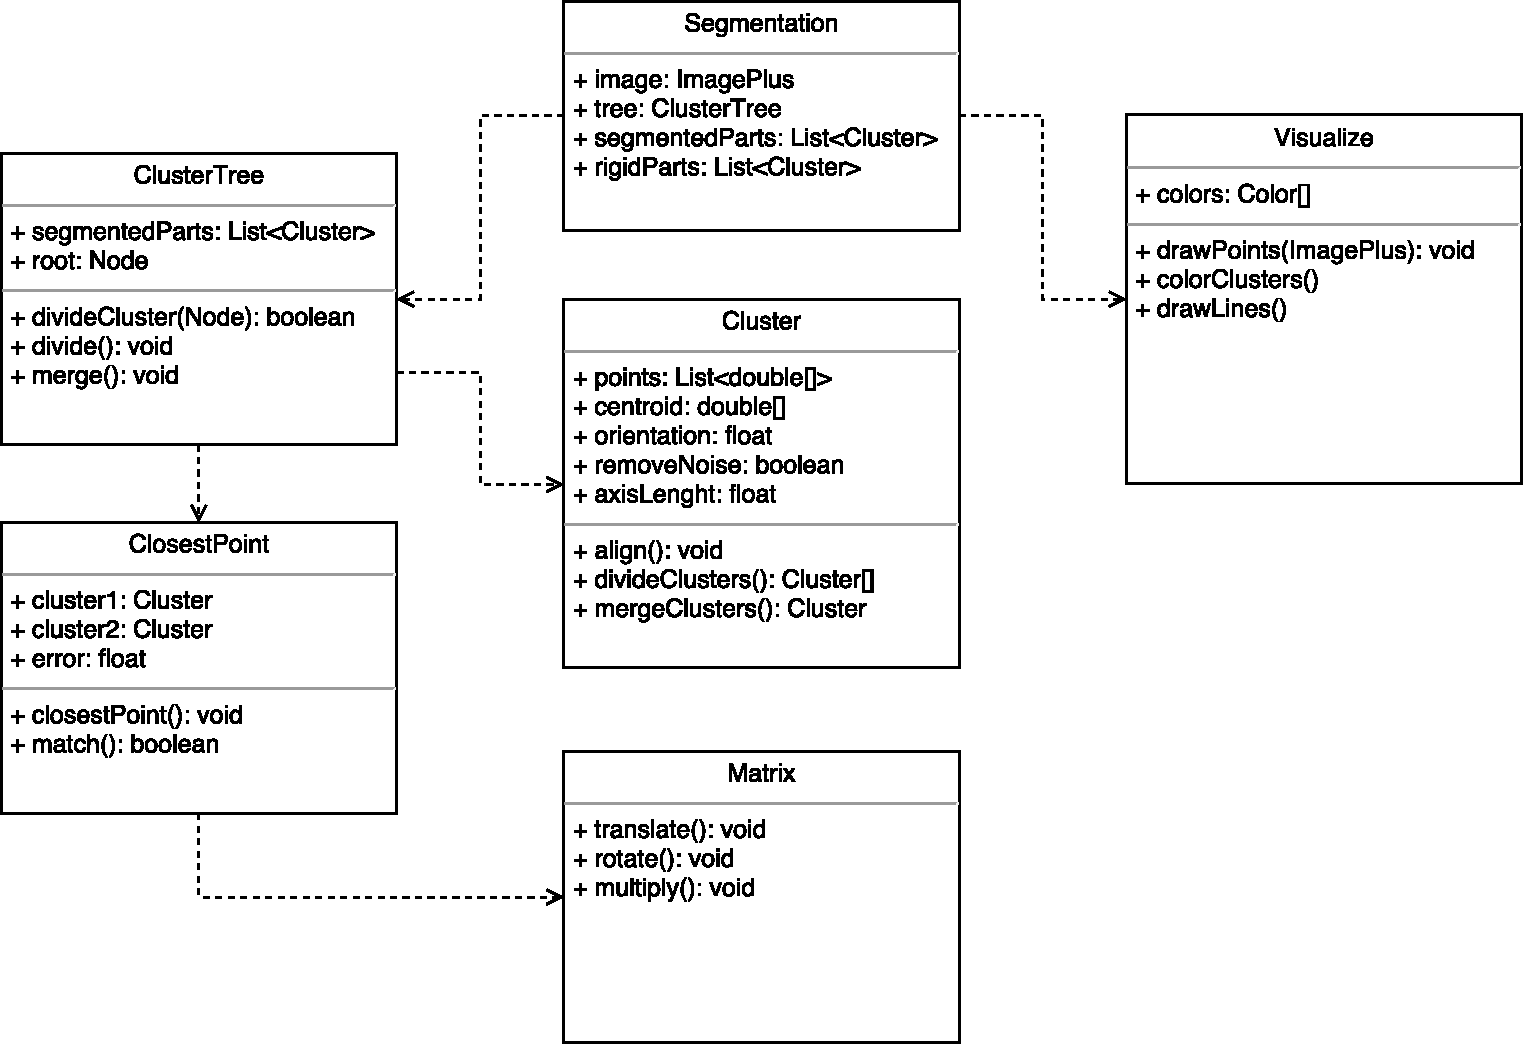
\includegraphics[width=0.8\linewidth]{SegmentationUML}
	\caption{UML diagram of the classes related to the implementation of the algorithm.}
	\label{fig:UML}
\end{figure}

\subsection{Region growing}
\label{RegionGrowing}
One main algorithm to remove outliers is the region growing from unclustered points given as input from a mesh $M$ (see algorithm \ref{alg:noiseRemoval}).

\begin{algorithm}[tbp]
	\label{alg:noiseRemoval}
	\caption{Noise removal of an input point mesh $M$ in form of a set of unclustered points $\{\boldsymbol{u}_1,\ldots,\boldsymbol{u}_n\}$ by region growing. The first point of $M$ is used as seed and grows a cluster $C_{current}$ by iteratively adding neighboring points located inside a threshold $\tau$. Once, all points have been examined, the largest cluster $C_{max}$ is returned and defined as articulated object to be segmented.}
	
	\begin{algorithmic}[1]     % [1] = all lines are numbered
		\Procedure{RemoveNoise}{$M$} 
		\State $M = \{\boldsymbol{u}_1,\ldots,\boldsymbol{u}_n\}$
		\State $\mathit{C_{max}} \gets ()$
		\State $\mathit{C_{current}} \gets ()$
		\State $n \gets \mathit{sizeOf}(M)$
		\State $m \gets \mathit{sizeOf}(C_{current})$
		
		\While {$n$ > 0}
		\State $\mathit{c_{current}} \gets \mathit{c_{current}} + \boldsymbol{u}_1$
		\For{$i = 1,\ldots,m$}
		\State $M \gets M - C_{current}$
		\For{$j = 1,\ldots,n$}
		\If {\Call{$d$}{$\boldsymbol{p}_i, \boldsymbol{u}_j}< \tau$}
		\State $C_{current} \gets C_{current} + \boldsymbol{u}_j$
		\EndIf
		\EndFor
		\EndFor
		\State $M \gets M - C_{current}$
		\If{$m > \mathit{sizeOf}(C_{max})$}
		\State $C_{max} \gets C_{current}$
		\EndIf
		\State $C_{current} \gets ()$
		\EndWhile
		\State\Return $C_{max}$
		\EndProcedure	
	\end{algorithmic}
\end{algorithm}
%%
\subsection{PCA}
One main factor for subdividing a cluster $C_i$ is the computation of its secondary axis, which represents the divider. To simplify the segmentation of $C_i$ into a left and right sub cluster, it is horizontally aligned. This is achieved by taking advantage of a rotation Matrix with the negative orientation of the cluster (see section \ref{Subdividing}). As a first step, the cluster is translated that the desired rotation point (which is the centroid of the cluster) is located at the origin of coordinates. After applying a rotation matrix, applying the negative orientation, the cluster is translated back to its initial position.

\begin{lstlisting}
public List<ClusterPoint> alignAxis(double orientation) {
	points = Matrix.translate(points, -centroid.getX(), -centroid.getY());
	points = Matrix.rotate(points, orientation);
	points = Matrix.translate(points, centroid.getX(), centroid.getY());
	orientation = 0;
	
	return points;
}
\end{lstlisting}

As a consequence, the secondary axis going through the cluster's centroid is vertically aligned. For the subdividing the x-coordinate of each point from the cluster to be divided is compared to the centroid's x-coordinate.

\begin{lstlisting}
for (ClusterPoint point : points) {
	if (point.getX() <= centroid.getX()) {
		left.add(point);
	} else {
		right.add(point);
	}
}
\end{lstlisting}

\subsection{Cluster tree}
\label{tree}
The subdividing of the clusters $C_1$ and $C_2$ is realized by a depth-first approach in a tree storing associated clusters in its nodes. Consequently, $C_1$ and $C_2$ represent the root and are subdivided from the left to the right. A node $N$ of the tree contains two related clusters $C_{1,i}$ and $C_{2,i}$, where $i$ defines whether the node is a left ($i=1$) or right ($i=2$) node of the parent. The actual decision maker of the algorithm is the registration (see section \ref{Registration}) of the two clusters of a node. The resulting error $e_{avg}$ decides whether to clusters match and subsequently need to be further subdivided.

\begin{lstlisting}
public List<Cluster[]> subdivide(Node node) {
	registration = new Registration(node.cluster[0], node.cluster[1]);

	if (!registration.match()) {
		split(node);
		subdivide(node.left);
		subdivide(node.right);
	} else {
		subclusters.add(node.clusters);
	}

	return subclusters;
}
\end{lstlisting}
In case of further subdividing, a Node $\mathit{left}$, containing the clusters $C_{1,i,1}$ and $C_{2,i,1}$, as well as a Node $\mathit{right}$, containing the clusters $C_{1,i,2}$ and $C_{2,i,2}$ origin. If two associated clusters $C_{1,i,j}$ and $C_{2,i,j}$ in a Node $N_i$ match, no further subdividing is performed. The resulting leaves of the tree are the final matching sub clusters and stored in a list $\mathcal{L} = (L_{1,1},L_{2,1},\ldots,L_{1,m},L_{2,m})$ from left to right (see algorithm \ref{subdivide}). By applying a depth-first approach, the matching clusters stored in the list are  actual neighboring clusters in $C_1$ and $C_2$. As a result, the adjacent sub clusters from $\mathcal{L}$ can be verified to be merged (see algorithm \ref{merging}). Figure \ref{fig:clusterTree} illustrates the subdividing step and merging in form of a \texttt{ClusterTree} and its resulting leaves.
%%
\begin{algorithm}[tbp]
	\caption{Recursive subdividing of two clusters $C_1$ and $C_2$, in the form of a Node $\mathit{N}$ in a \texttt{ClusterTree}, into matching sub clusters. The registration is performed on two corresponding clusters in $\mathit{N}$ to verify them to match, in which case they are stored in a list of matching sub clusters. Otherwise, if the two clusters do not match, they are further subdivided. The list with all matching sub clusters is returned once the subdivide algorithm terminates.}
	\label{alg:subdivide}
	
	\begin{algorithmic}[1]     % [1] = all lines are numbered
		\label{clusterTree}
		\Procedure{ClusterTree}{$\mathit{C_1}, \mathit{C_2}$}
		
		\State $L \gets ()$
		\State $\mathit{left} \gets \mathit{nil}$
		\State $\mathit{right} \gets \mathit{nil}$
		\State $N \gets \langle C_1, C_2, \mathit{left}, \mathit{right}\rangle$
		\State $L \gets \Call{Subdivide}{N}$
		\State $P \gets \Call{MergeClusters}{L}$
		
		\EndProcedure
	\end{algorithmic}
	
	\begin{algorithmic}[1]     % [1] = all lines are numbered
		\label{subdivide}
		\Procedure{Subdivide}{$N$}
		
		\If {$\Call{match}{C_1(N)}, C_2(N)$}
		\Comment{Apply ICP on two clusters}
		\State $L \gets L + (N)$
		
		\Else
		\State $\mathit{left}(N) \gets \Call{Split}{N}$
		\State $\mathit{right}(N) \gets \Call{Split}{N}$
		\Comment{Split the cluster into a left and right side}
		\State \Call{Subdivide}{$\mathit{left}(N)$}
		\State \Call{Subdivide}{$\mathit{right}(N)$}
		\Comment{Recall the algorithm with sub clusters}
		\EndIf
		
		\State\Return $L$
		\Comment{Return all sub clusters after termination.}
		\EndProcedure
		
	\end{algorithmic}
\end{algorithm}
%%
\begin{algorithm}[tbp]
	\caption{Merging of the sub clusters $\mathit{L} = ((L_{1,1}, L_{2,1}),\ldots,(L_{1,m}, L_{2,m}))$, resulting from algorithm \ref{alg:subdivide} in the order of being stored, to rigid parts $\mathcal{P}$. Verify the matching of merged adjacent clusters $L_{i,j}$ and $L_{i,j+1}$ from $C_1$ and $C_2$. The merging is continued until no matching is performed. In this case the last merged cluster pairs are stored as rigid parts $P_1$ and $P_2$. The algorithm then continues with the next cluster pair in the list and terminates if all pairs have been traversed. The list with all detected rigid parts $\mathcal{P}$ is returned.}
	\label{alg:merging}
	
	\begin{algorithmic}[1]     % [1] = all lines are numbered
		\label{merging}
		
		\Procedure{MergeClusters}{$L$} 
		\State $P \gets ()$
		\State $P_1 \gets L_{1,1}$
		\State $P_2 \gets L_{2,1}$
		\State $n \gets \mathit{sizeOf}(L)$
		
		\For{$i = 2,\ldots,n$}
		\State $\mathit{merge_1} \gets \Call{Merge}{P_1, L_{1,i}}$
		\State $\mathit{merge_2} \gets \Call{Merge}{P_2, L_{2,i}}$
		
		\If {\Call{match}{$merge_1$, $merge_2$}}
		\Comment{Apply ICP on two merged clusters}
		\State $\mathit{P_1} \gets merge_1$
		\State $\mathit{P_2} \gets merge_2$
		\Comment{Continue merging with merged clusters}
		\Else
		\State $P \gets P + (P_1, P_2)$
		\State $P_1 \gets L_{1,i}$
		\State $P_2 \gets L_{2,i}$
		\Comment{Initiate merging with current clusters}
		\EndIf
		\EndFor
		\State $P \gets P + (merge_1, merge_2)$
		\State\Return $P$
		\EndProcedure	
	\end{algorithmic}
\end{algorithm}
%%
\begin{figure}[H]
	\centering\small
	\begin{tabular}{cc}
		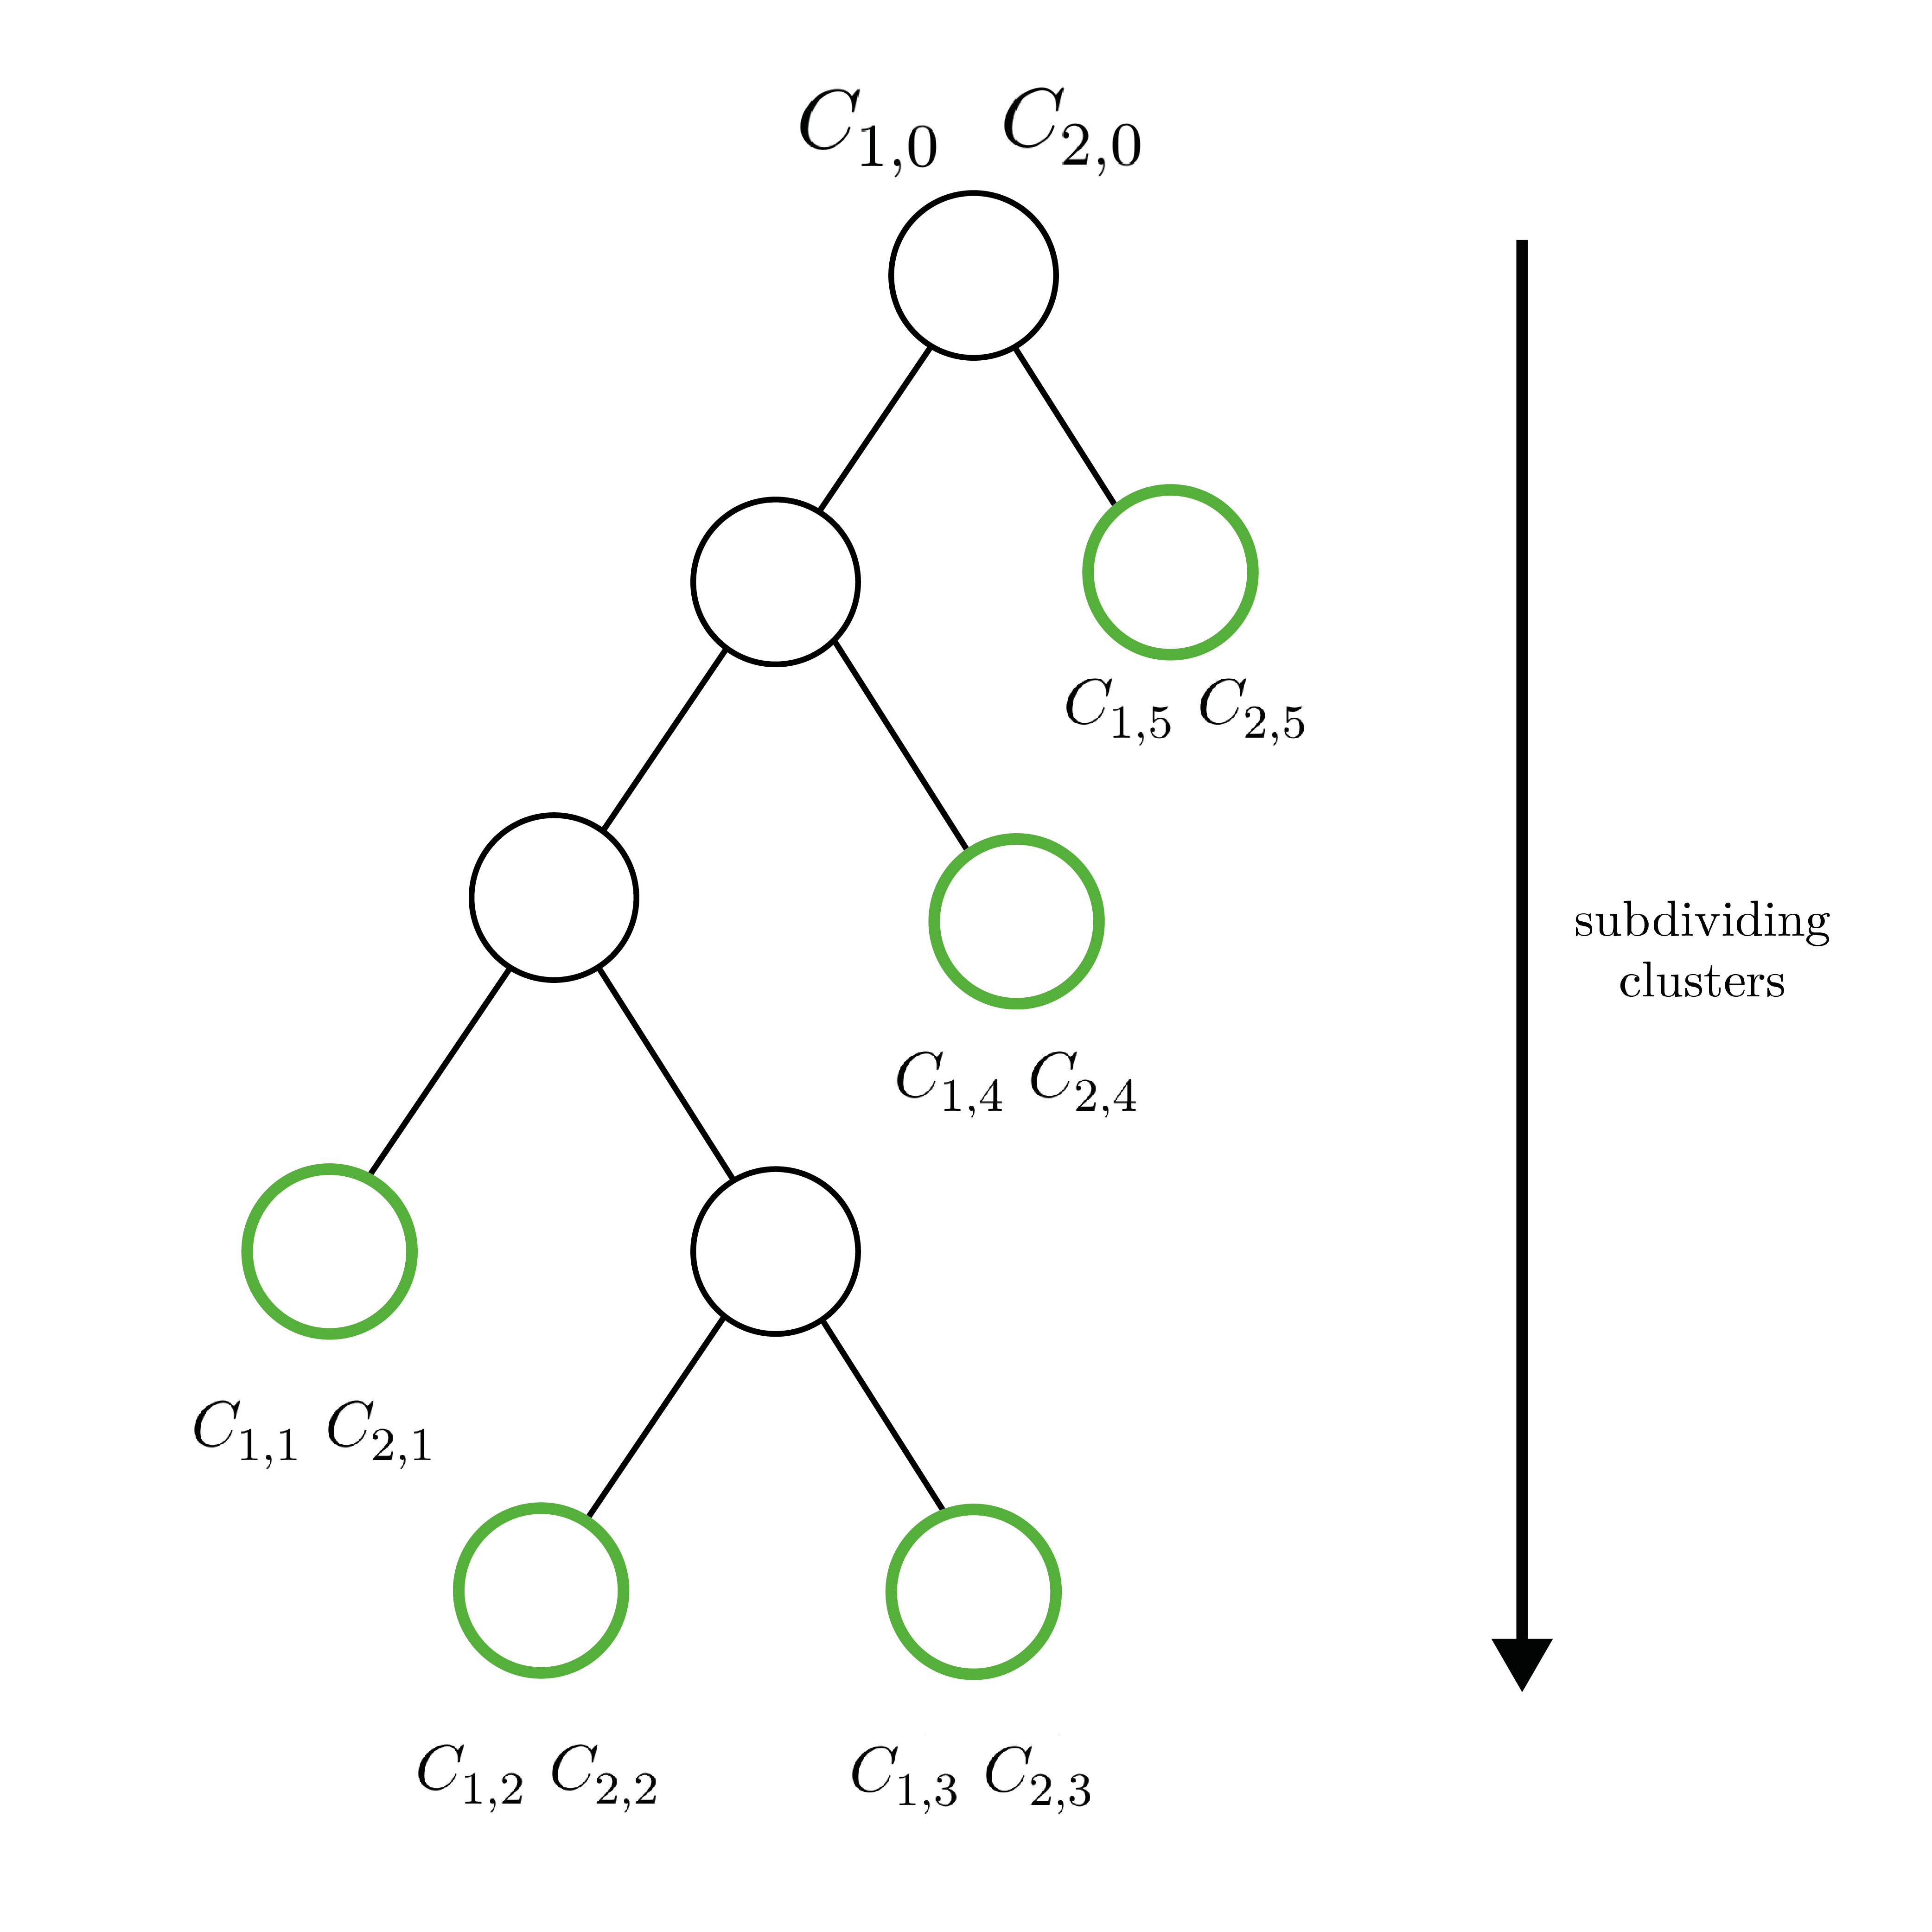
\includegraphics[width=0.45\textwidth]{IllustrationTree} &	
		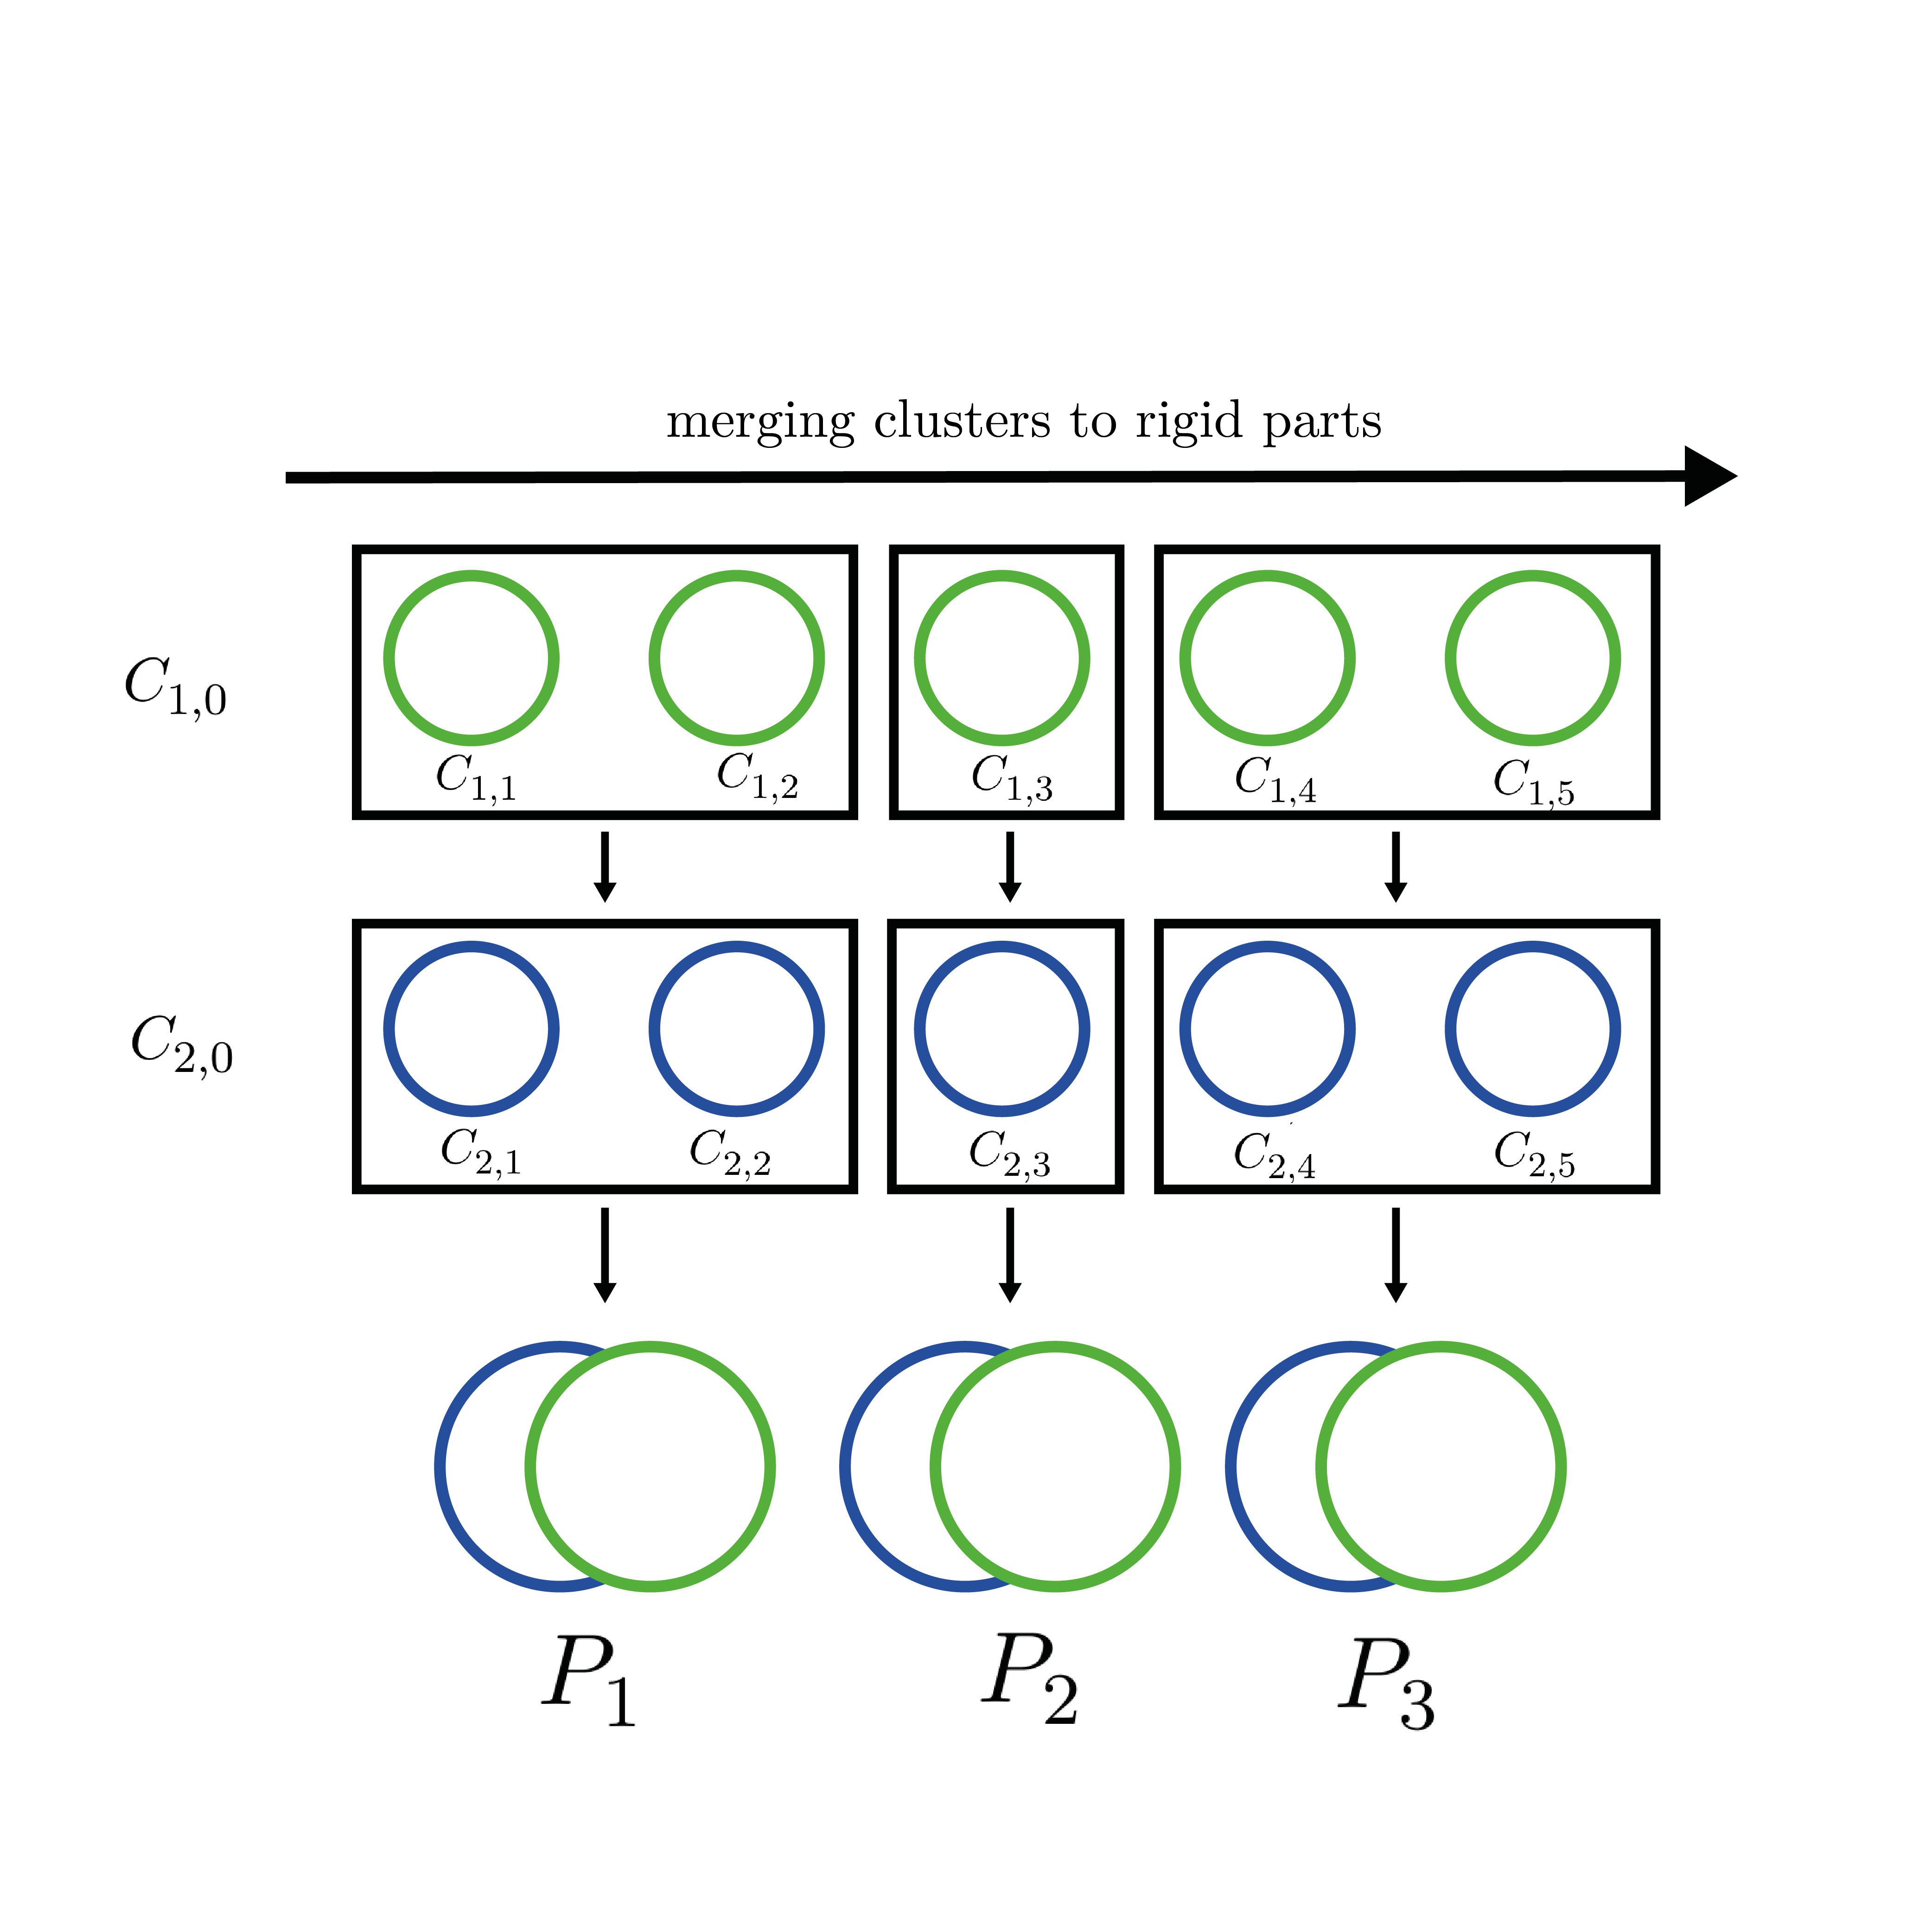
\includegraphics[width=0.45\textwidth]{ClusterChain}
		\\
		(a) & (b) 
	\end{tabular}
	\caption{Subdividing of $C_1$ and $C_2$ into matching clusters by a depth-first approach in a tree. The Subdividing terminates if all sub clusters of $C_1$ and $C_2$ match when applying the ICP~(a). Detecting rigid parts of $C_1$ and $C_2$ by iteratively merging adjacent clusters of $\mathcal{L}$ that merged clusters still match~(b).} 
	\label{fig:clusterTree}
\end{figure}
%%
\subsection{Registration}
\label{Registration}
The \texttt{Registration} aims to compute a rigid transformation on the reference points from cluster $C_i$ which results in the lowest matching error $e$ by comparing the distance to the target points of the input cluster $C_j$. For an initial alignment, $C_i$ and $C_j$ are similarly oriented and their centroids $c_i$ and $c_j$ are translated that they overlap. Then, iteratively the best possible alignment of $C_i$ and $C_j$ is aimed for. As a first step, the sorted associated points for the reference points are computed. This is achieved by seeking the closest neighbor for each reference point $p_i$ in terms of the smallest euclidean distance $d(\boldsymbol{p}_i,\boldsymbol{p}_j)$ to a target point $p_j$. As a next step, Procrustes fitting \cite{procrustesFitting} is applied on the reference points and its associated target points. Procrustes fitting tries to enforce a rigid transformation between two corresponding, sorted point lists which results in the an error $e_{PF}$. In case of a smaller error $e_{PF}$ than from previous iterations the reference and associated points are stored as final transformed and target points. Additionally, the smallest error is adjusted. By applying the computed transformations from Procrustes Fit, the iterative process initiates with updated reference points. It terminates if the two clusters finally match or the maximum number of iterations is reached. This is required, in order to avoid a infinite loop if the two clusters do not match.
%%
\begin{lstlisting}
while (!match() && iterations < MAX_ITERATIONS) {
	association = getAssociation(referencePoints, targetPoints);
	
	pro.fit(referencePoints, association);
	tmp_error = pro.getError();
	
	if (tmp_error < error) {
		error = tmp_error;
		finalTargetPoints = association;
		finalReferencePoints = referencePoints;
	}
	
	ClusterPoint c = calculateCentroid(finalReferencePoints);
	
	referencePoints = Matrix.translate(referencePoints, -c.getX(), -c.getY());
	referencePoints = Matrix.rotate(referencePoints, Math.acos(pro.getR().getEntry(0, 0)));
	referencePoints = Matrix.translate(referencePoints, c.getX() + pro.getT().getEntry(0), c.getY() + pro.getT().getEntry(1));
	
	iterations++;
}
\end{lstlisting}

The average error per point $e_{avg}$ is calculated from the $e_PF$ which represents the total squared error for an estimated fit. Thereby, it is divided by the total number of reference points. 
%
\begin{lstlisting}
public boolean match() {
	double errorPerPoint = error / amountPoints;

	if (errorPerPoint < errorThreshold) {
		return true;
	}
	
	return false;
}

\end{lstlisting}
%%
\section{Results}
At first, the implemented algorithm was applied on two point clouds of an articulated object composed of two rigid parts. The segmentation results are directly dependent on the matching error threshold $\tau$ which can bee seen on table \ref{table:segmentation_results}. The higher the threshold $\tau$, the less clusters and subsequently rigid parts can be detected. The reason is that two clusters are more likely to match and are not further subdivided. The lower $\tau$, the more clusters and rigid parts will be detected, as clusters require further subdividing in order to match. Figure \ref{fig:2rigidParts} and figure \ref{fig:3rigidParts} show the segmentation of two simple objects into their rigid parts which are linked like a chain. For those objects, with a error threshold $\tau = 5.0$ the right number of rigid parts is detected. However, the segmentation position does not correspond to the actual joint of $C_1$ and $C_2$. The reason is, that the average error $e_{avg}$ is computed without any weighting of points. Especially points located near a joint need to be treated cautiously.
The segmentation into rigid parts is also apparent, when visualizing the point registration between $C_1$ and $C_2$ (see figure \ref{fig:ICPResults}). Two associated points from $C_1$ and $C_2$ are thereby linked with green lines. Comparing the registration results before and after a segmentation into rigid parts clearly shows, that the registration after segmentation results in a lower matching error $e$.
%%	
\begin{table}
	\centering\small
	\begin{tabular}{ |c|c|c|c| } 
		\hline
		Rigid parts & $\tau$ & detected clusters & detected rigid parts \\
		\hline
		& 3 & 21 & 14 \\ 
		2& 5 & 3 & 2 \\
		& 7 & 2 & 2 \\
		\hline
		& 4 & 38 & 31 \\ 
		3 & 6 & 4 & 3 \\
		& 8 & 3 & 3 \\
		\hline
		& 6 & 35 & 26 \\ 
		4 & 7 & 3 & 3 \\
		& 8 & 3 & 3 \\
		\hline
	\end{tabular}
	\caption{Segmentation results}
	\label{table:segmentation_results}
\end{table}
%%
\begin{figure}[H]
	\centering\small
	\begin{tabular}{cc}
		\fbox{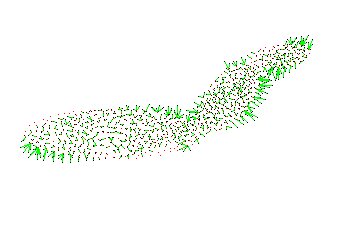
\includegraphics[width=0.45\textwidth]{results/non-rigid_3parts_associations}} &	
		\fbox{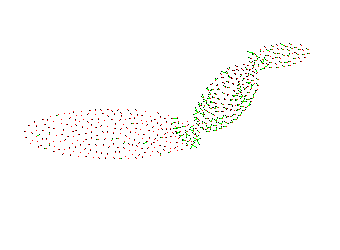
\includegraphics[width=0.45\textwidth]{results/rigid_3parts_associations}} 
		\\
		(a) & (b) 
	\end{tabular}
	\caption{Registration of $C_1$ and $C_2$ before the segmentation into rigid parts (a) and after the segmentation (b).} 
	\label{fig:ICPResults}
\end{figure}
%%
As the main goal is to segment a human-like articulated object into its rigid parts, a more complex mesh was taken as input. Contrary to the previous input object, a rigid part is linked to multiple other rigid parts. Figure \ref{fig:4rigidParts} shows the segmentation results.
%%
\begin{figure}
	\centering\small
	\begin{tabular}{@{}c@{\hspace{2mm}}c@{}} % mittlerer Abstand = 12mm
		\fbox{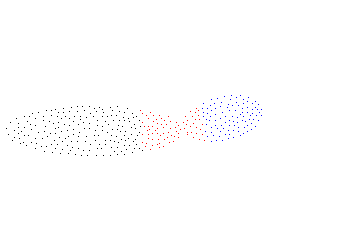
\includegraphics[width=.40\textwidth]{results/2_1parts_clusters_2th}} &
		\fbox{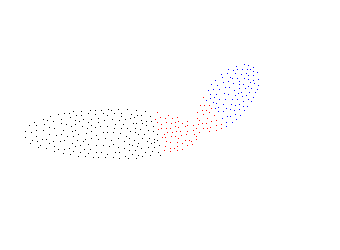
\includegraphics[width=.40\textwidth]{results/2_2parts_clusters_2th}} 
		\\
		(a) & (b)
		\\[4pt]	%vertical extra spacing (4 points)
		\fbox{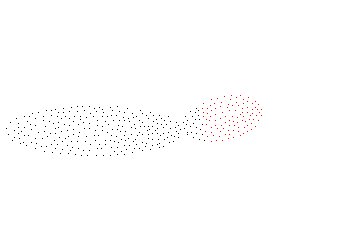
\includegraphics[width=.40\textwidth]{results/2_1parts_rigidParts_2th}} &
		\fbox{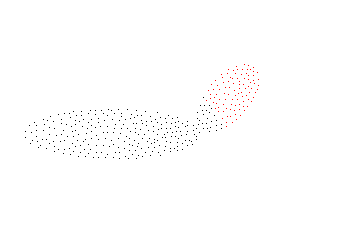
\includegraphics[width=.40\textwidth]{results/2_2parts_rigidParts_2th}} 
		\\
		(c) & (d)
	\end{tabular}
	\caption{Taking a Mesh $M$ in two poses with only two rigid parts as input, with a threshold $\tau = 5$, 3 clusters are detected in $C_1$~(a) and $C_2$~(b),
		which results in 2 rigid parts in $C_1$~(c) and $C_2$~(d).}
	\label{fig:2rigidParts}
\end{figure}
%%
\begin{figure}
	\centering\small
	\begin{tabular}{@{}c@{\hspace{2mm}}c@{}} % mittlerer Abstand = 12mm
		\fbox{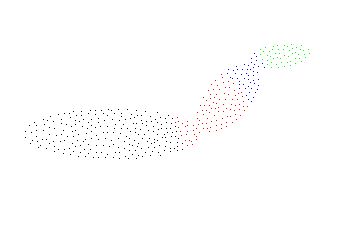
\includegraphics[width=.40\textwidth]{results/3_1parts_clusters_2th}} &
		\fbox{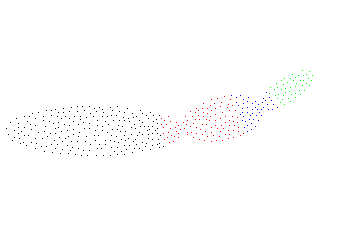
\includegraphics[width=.40\textwidth]{results/3_2parts_clusters_2th}} 
		\\
		(a) & (b)
		\\[4pt]	%vertical extra spacing (4 points)
		\fbox{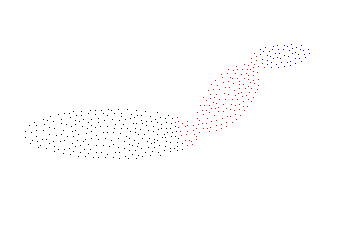
\includegraphics[width=.40\textwidth]{results/3_1parts_rigidParts_2th}} &
		\fbox{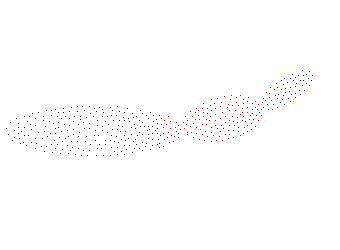
\includegraphics[width=.40\textwidth]{results/3_2parts_rigidParts_2th}} 
		\\
		(c) & (d)
	\end{tabular}
	\caption{Taking a Mesh $M$ in two poses with three rigid parts as an input, with a threshold $\tau = 6$, 4 clusters are detected in $C_1$~(a) and $C_2$~(b),
		which results in 3 rigid parts in $C_1$~(c) and $C_2$~(d).}
	\label{fig:3rigidParts}
\end{figure}
%%		
In case of a more complex object, the simple segmentation algorithm fails. Although varying threshold $\tau$ for the matching, there are either too many or few rigid parts detected. When using $\tau = 7$ (see figure \ref{fig:4rigidPartsHighTH}) only 3 clusters and rigid parts can be detected. By decreasing $\tau$ to 6 (see Figure \ref{fig:4rigidParts}), further subdividing is done, which leads to a too high number of rigid parts and clusters.
%%
\begin{figure}[H]
	\centering\small
	\begin{tabular}{cc}
		\fbox{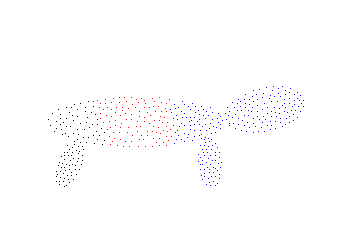
\includegraphics[width=0.45\textwidth]{results/4_1parts_clusters_rigidParts_7th}} &	
		\fbox{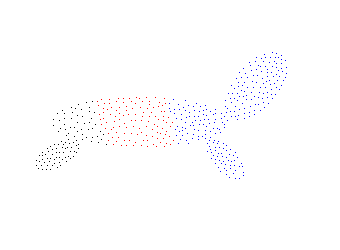
\includegraphics[width=0.45\textwidth]{results/4_2parts_clusters_rigidParts_7th}} 
		\\
		(a) & (b) 
	\end{tabular}
	\caption{Taking a more complex Mesh $M$ in two poses with four rigid parts as an input, with a threshold $\tau = 7$, 3 clusters and rigid parts can be detected in $C_1$~(a) and $C_2$~(b).} 
	\label{fig:4rigidPartsHighTH}
\end{figure}
\begin{figure}[H]
	\centering\small
	\begin{tabular}{@{}c@{\hspace{2mm}}c@{}} % mittlerer Abstand = 12mm
		\fbox{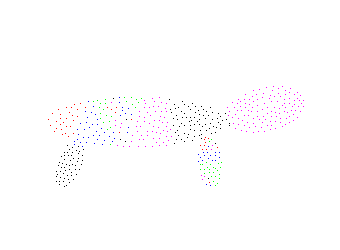
\includegraphics[width=.40\textwidth]{results/4_2parts_clusters_6th}} &
		\fbox{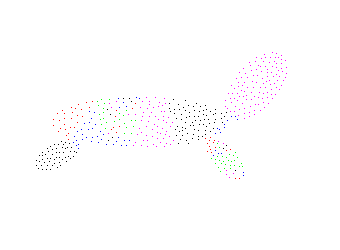
\includegraphics[width=.40\textwidth]{results/4_1parts_clusters_6th}} 
		\\
		(a) & (b)
		\\[4pt]	%vertical extra spacing (4 points)
		\fbox{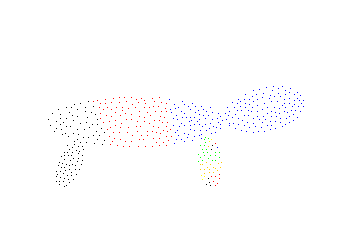
\includegraphics[width=.40\textwidth]{results/4_1parts_rigidParts_6th}} &
		\fbox{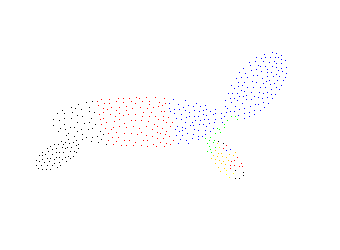
\includegraphics[width=.40\textwidth]{results/4_2parts_rigidParts_6th}} 
		\\
		(c) & (d)
	\end{tabular}
	\caption{Taking a more complex Mesh $M$ in two poses with four rigid parts as an input, with a threshold $\tau = 6$ , 35 clusters are detected in $C_1$~(a) and $C_2$~(b),
		which results in 26 rigid parts in $C_1$~(c) and $C_2$~(d).}
	\label{fig:4rigidParts}
\end{figure}	
The algorithm generally results in satisfying results for simple objects, whose rigid parts are linked like a chain. Still, the segmentation location is not accurate, which might be disposed by introducing weights to points located near a joint. For more complex object with a skeleton structure, e.g. an animal, where one rigid part is linked to more than two rigid parts, this simple implementation fails. In this case, another approach has to be implemented, as a skeleton structure is more complex to extract than a simple chain structure.

\section{Possible improvements}
In case of articulated objects with a skeleton structure, the segmentation algorithm in its simple form fails. The main issues can be summarized as the following:
%%
\begin{enumerate}
	\item By linearly subdividing a cluster $C_i$ along its secondary axis more than two sub clusters can origin. In this case a sub cluster might consist of points located far apart from each other which distorts the segmentation into rigid parts.
	\item Clusters being compared might not contain the same number or not even the same corresponding points as the dividing only builds on the secondary axis as divider. In case of great transformation differences of corresponding rigid parts the position of the computed secondary axis and subsequently the sub clusters may considerably differ from each other.
	\item The segmentation procedure results only into approximated rigid parts. The reason is that sub clusters might match even if a number of points considerably contribute to a higher average matching error. Points with a quite low error will compensate those outliers and as a result a successful match is detected. Still, there might be a better segmentation with less points.
	\item In case of detecting two matching clusters being a part of a rigid part, no further operations are directly conducted in order to find the actual rigid part they belong to. It is anticipated to be detected in a later step by merging neighboring sub clusters.
	\item By further sub dividing clusters, the merging becomes more difficult, as the clusters are scattered next to each other and it is difficult to guarantee that stored adjacent clusters are associated in two different poses.
\end{enumerate}
%%
Regarding the listed issues being responsible for the unsuccessful results for articulated objects, the initial approach needs to be extended. 

\subsection{Assuring corresponding, similar clusters}
During the segmentation of an object in two different poses, there is the general case that the divided parts being compared do not contain the same number or even additional points being part of an actual different cluster (see issues 1 and 2). As this state might come to undesirable matching errors, parts with the same sizes could be generated by region growing. This can be e.g. implemented by starting the clustering with two points farthermost from the centroids of two input clusters. By growing regions with the same size of points presumably similar clusters can be compared. Additionally, the detection of multiple clusters is considered as those are treated individually.

\subsection{Matching error}
The current matching error considers the average error per point where considerable close point correspondences might compensate points actually belonging to a neighboring rigid part. The goal should be to focus only on the best point correspondences as an indicator where the segmentation has to take place, namely in the region of a high number of outliers. By introducing weights to points with a high distance the error $e$ would be more expressive as instead of compensating those points a further segmentation will have to be conducted. Being able to locate points obviously not corresponding to a rigid part the segmentation might proceed by selecting the best matching points instead of subdividing and merging the rigid part in a later step (see issues 3 and 4).

\subsection{Initial alignment of largest rigid part}
The most crucial deficit of the proposed algorithm is that it does not results in a successful segmentation regarding complex articulated objects, whose rigid parts are not composed like a chain. Instead, a rigid part may be linked to multiple rigid parts. As a result, the objects are too complex to be linearly subdivided. One improvement proposition is thereby the initial alignment of the object, that the largest rigid part is aligned. Then, recursively linked parts of this largest rigid part are detected. A similar approach was taken during the recursive algorithm from Guo et al \cite{guo2016correspondence} (see section \ref{LRP}). The main idea is to apply a modified ICP with the goal to align the largest possible cluster. Point correspondences of two input clusters $C_i$ and $C_j$ are initially achieved by aligning them by means of a similar orientation. Following, corresponding points of $C_i$ and $C_j$ are only considered, if they are \textit{reciprocal} (see subsection \ref{functionalityLRP}). Furthermore, the euclidean distance between two cluster points $d(\boldsymbol{p}_i,\boldsymbol{p}_j)$ must be below a predefined threshold $\tau$. As a consequence, points being located far away from each other do not contribute to the alignment of $C_i$ and $C_j$ and are not stored as correspondence. Those are assumed to be small rigid parts with different transformations. The results are directly dependent on the extend of transformations of the two articulated clusters $C_1$ and $C_2$. The more different the transformations, the higher the changes that the initial alignment of the largest rigid part might fail. The reason is that the ICP expects a good starting alignment. It is assumed that the largest rigid part contributes most to the principal axis and the initial alignment. But in case of a considerable unbalance of the linked parts, the alignment of the LRP might shift in a certain direction and it might not be detected during the ICP. As a result the whole algorithm fails.

\begin{figure}
	\centering
	
\includegraphics[width=0.8\linewidth]{Placeholder}
	\caption{Detecting rigid parts of $C_1$ and $C_2$ by iteratively merging adjacent clusters of $\mathcal{L}$ that merged clusters still match.}
	\label{fig:ICPforLRP}
\end{figure}
%TODO: images of results + new datasets (hull)

\section{Outcome}
Although, some of the proposed optimizations are implemented, the overall segmentation results for complex objects did not considerable improve.  Still, the implementation of this linear approach allowed to acquire a significant knowledge gain in terms of the segmenting non-rigid objects into their rigid parts. The most relevant observation is that relying only on the coordinates of points is not sufficient for the segmentation of complex articulated objects, like humans. Additional point descriptors are required to detect reliable point correspondences between $C_1$ and $C_2$. The focus at this point is shifted to a feature-based approach (see chapter \ref{cha:FeatureApproach}).
